\documentclass[final, xcolor={dvipsnames}]{beamer}

\renewcommand\familydefault{\sfdefault} 
\usepackage[scaled]{helvet}

\usetheme{/inria-willow}

\usepackage{amsmath,amssymb}
\usepackage[english]{babel}
\usepackage[latin1]{inputenc}
\usepackage{booktabs}
\usepackage[orientation=portrait,size=a0,scale=1.2,debug]{beamerposter}
\usepackage[framemethod=TikZ]{mdframed}
\usepackage{adjustbox}
\usepackage{hyperref}

\def \postercolumnbreak {\vrule width 5pt height -2.5cm \hskip1cm}
\mdfdefinestyle{posterframe}{default,roundcorner=50pt, linewidth=10pt,innerbottommargin=50pt}
\mdfdefinestyle{posteremphasize}{default,linewidth=2pt, font=\large, backgroundcolor=red!10}%lightgray!30}

\title{ContextLocNet: Context-aware Deep Network Models \\for Weakly Supervised Localization}
\author{Vadim Kantorov, Maxime Oquab, Minsu Cho, Ivan Laptev}
\institute{INRIA / ENS, Paris}

\begin{document}
\begin{frame}[t,fragile]{} 
\begin{mdframed}[style = posterframe]

\leavevmode
\begin{columns}[t,onlytextwidth]

\begin{column}{.26\linewidth}
	 
	\begin{block}{Goal}
		%\begin{itemize}
			\begin{center}
			Localize objects with only image-level labels at train time, i.e. weakly supervised localization.
			\end{center}
			%\item Evaluated by detection mAP and CorLoc
		%\end{itemize}
		%\begin{center}
 		%	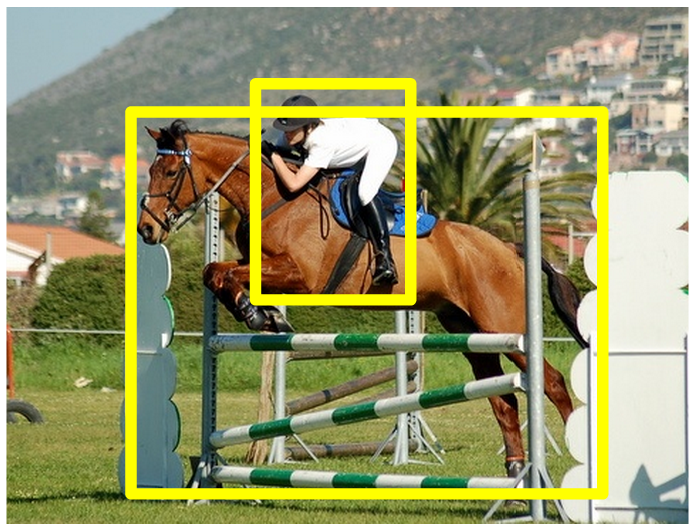
\includegraphics[width=.8\textwidth]{images/wsl}
		\begin{center}
 			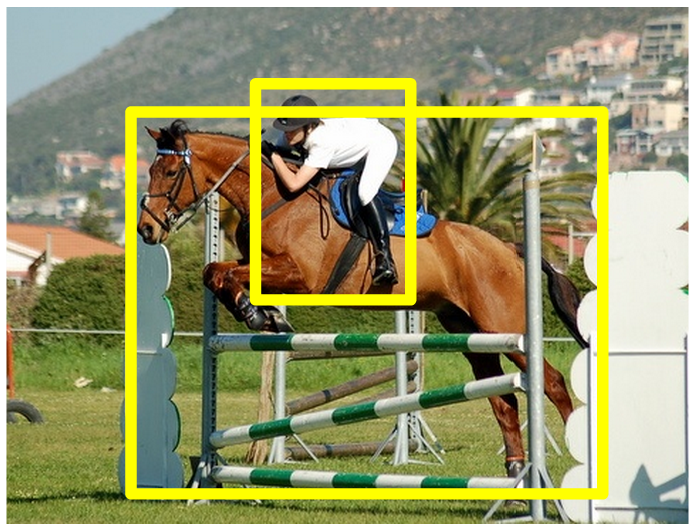
\includegraphics[width=.8\textwidth]{images/wsl}
			
			In train time: \textcolor{ForestGreen}{\checkmark} horse \textcolor{ForestGreen}{\checkmark}{person}
		\end{center}
		%	In train time: \textcolor{ForestGreen}{\checkmark} horse \textcolor{ForestGreen}{\checkmark}{person}
		%\end{center}
	\end{block}

	\begin{block}{Motivation}
		Weakly supervised localization often results in errors due to:
		\begin{itemize}
			\item shrinking to most discriminative parts
			\item expansion beyond object boundaries
		\end{itemize}
		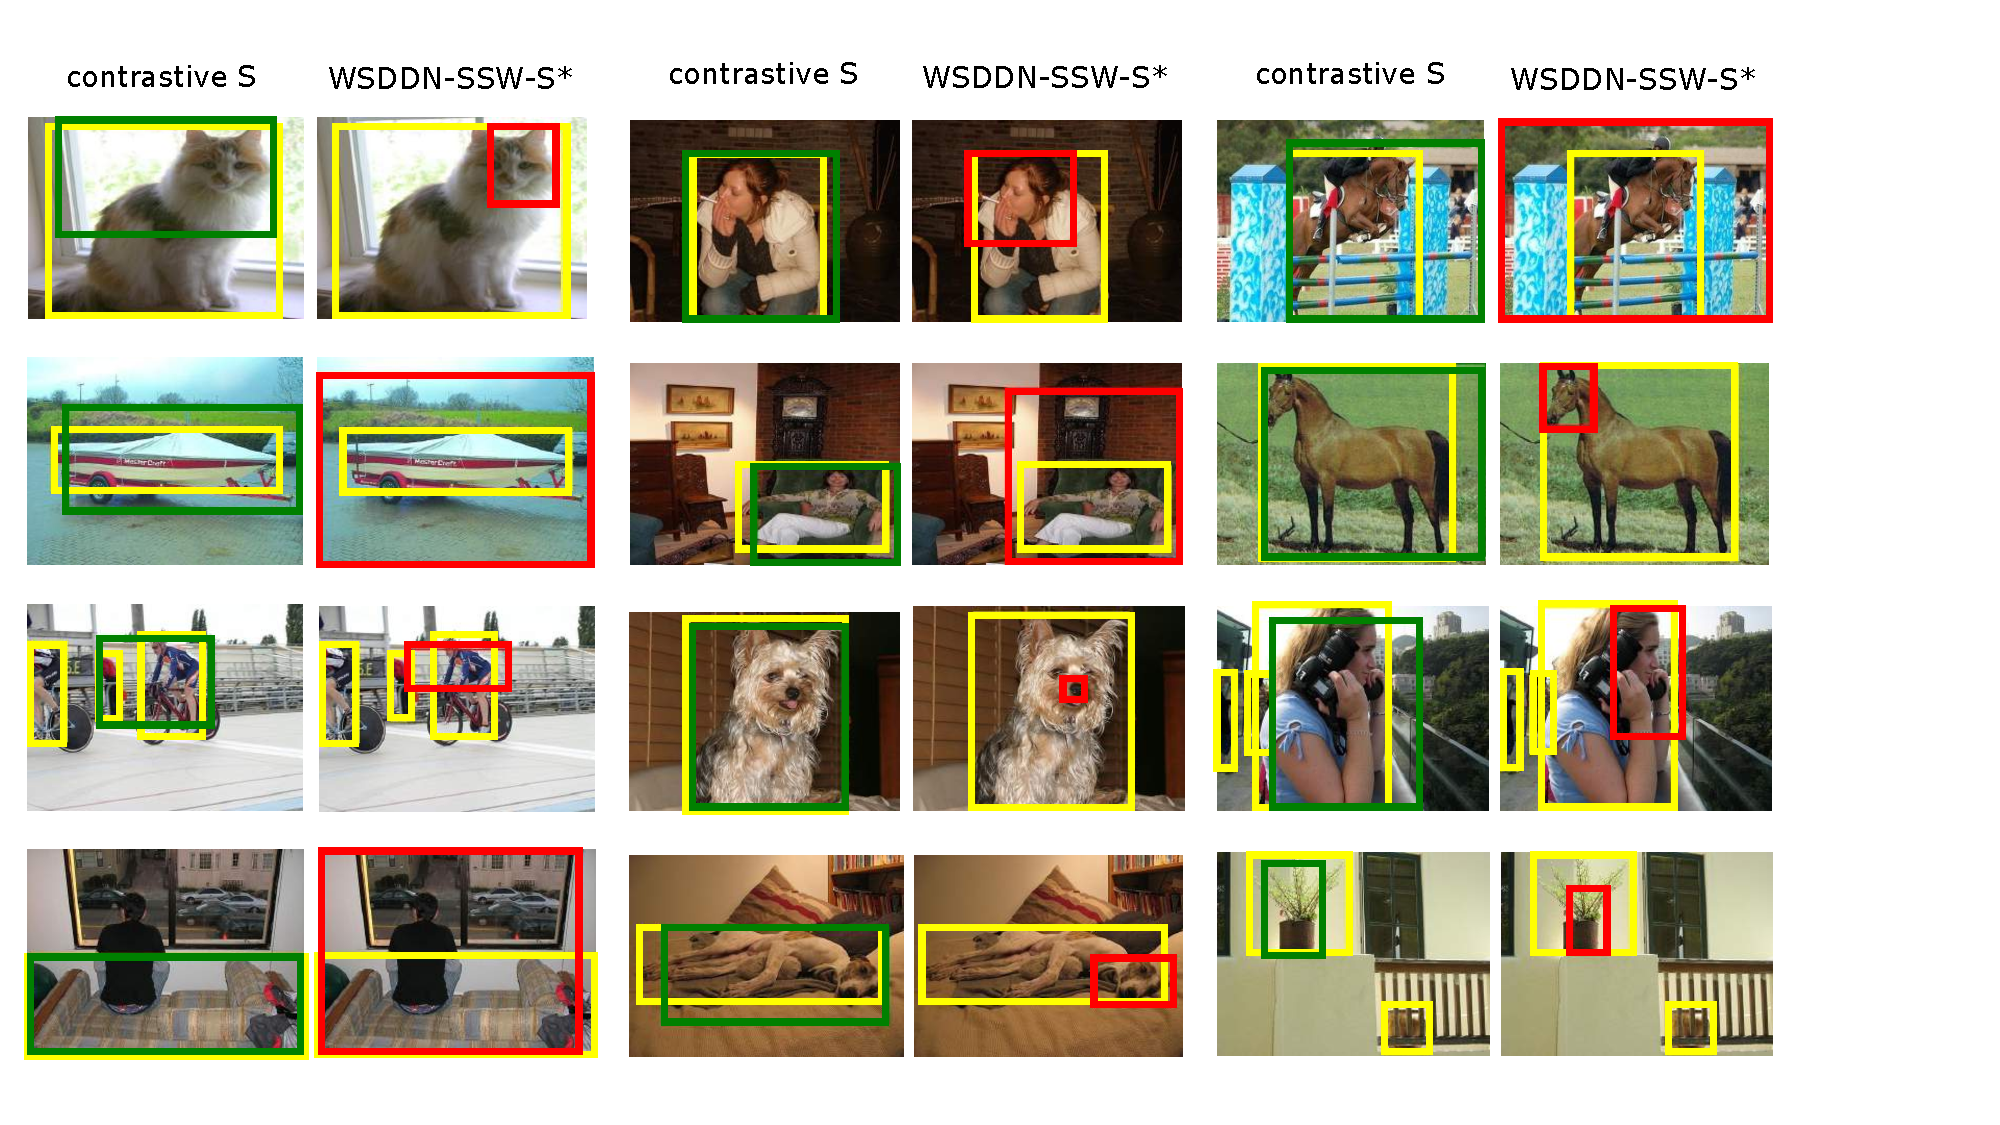
\includegraphics[trim = 5.2cm 13.5cm 23.8cm 2cm, clip, width=0.48\linewidth] {images/detectionresults_goodbad_1_compressed.pdf}
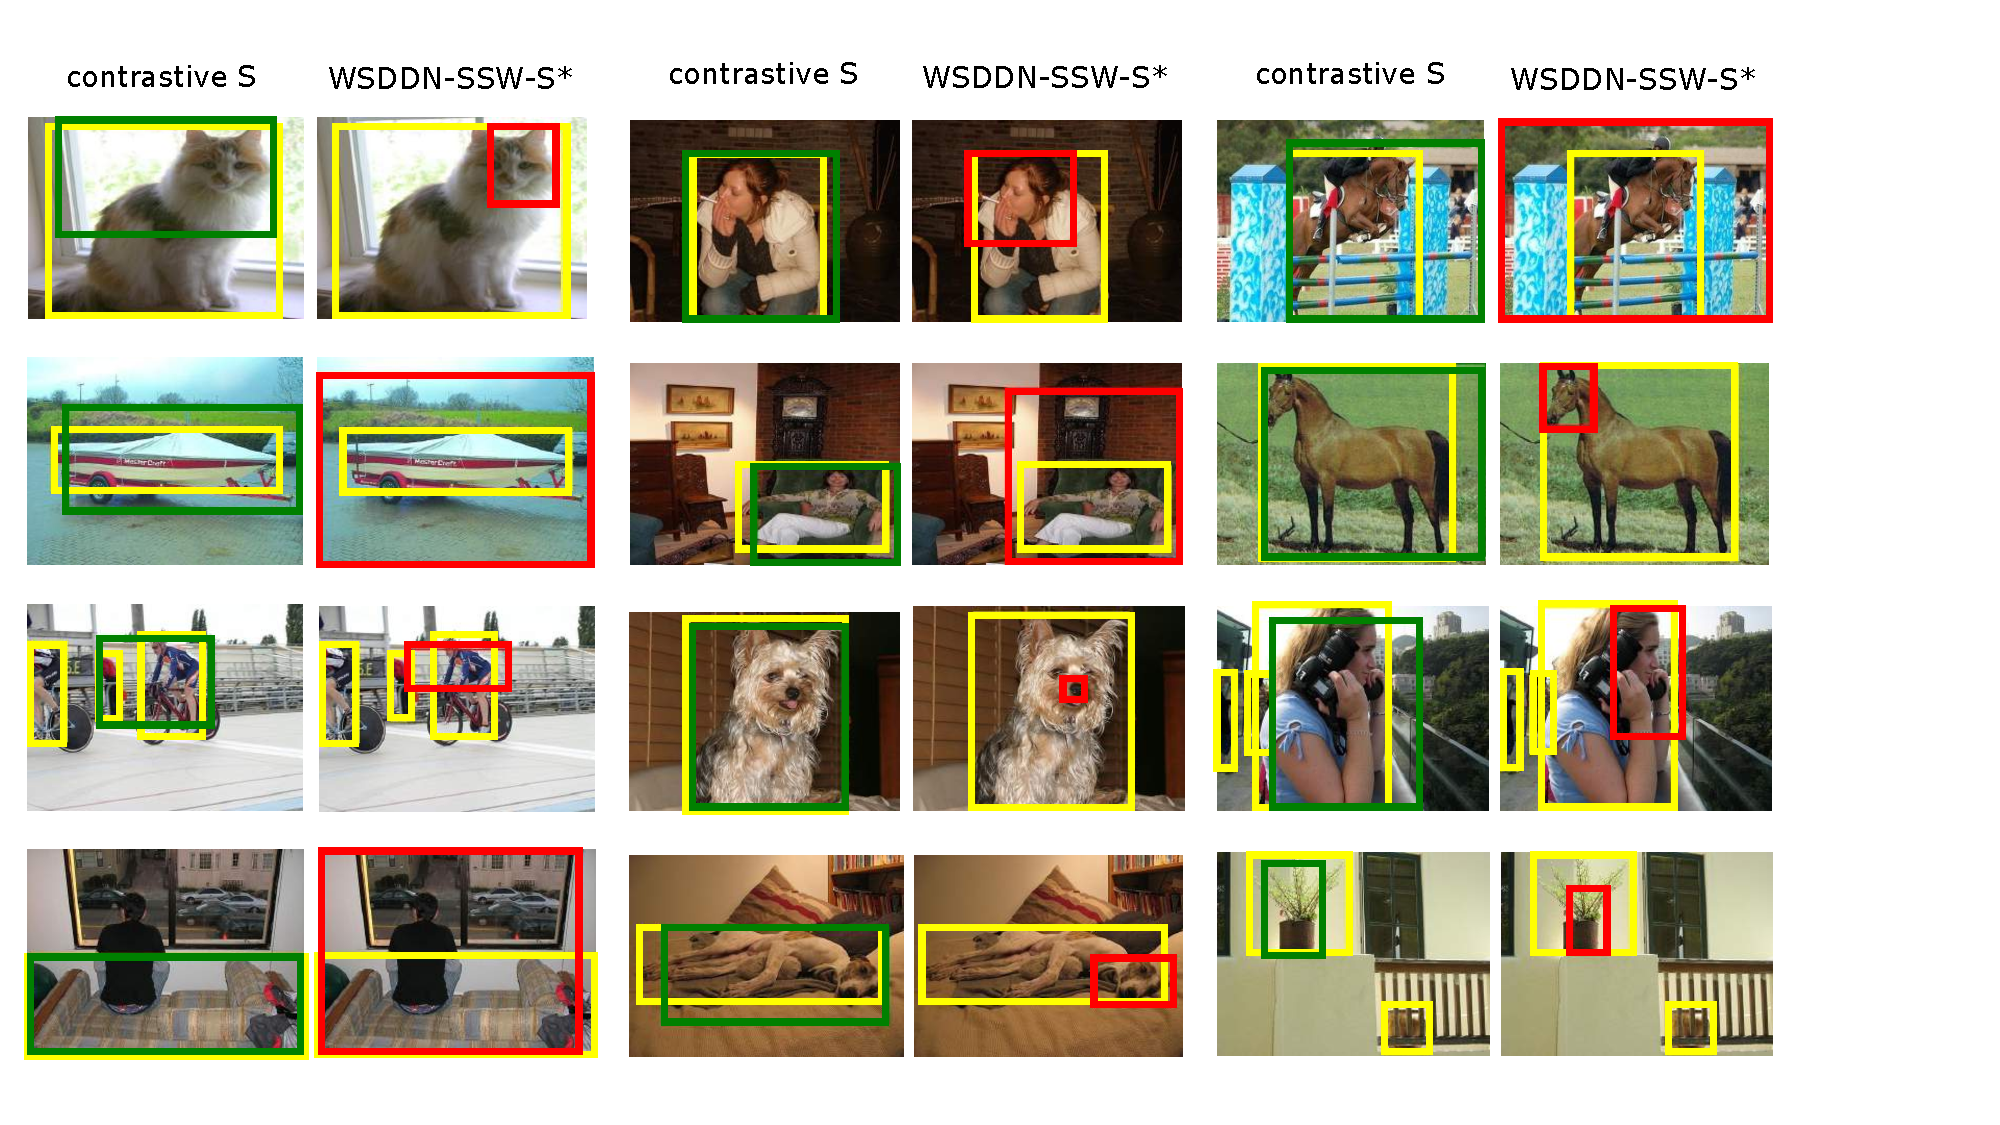
\includegraphics[trim = 5.2cm 9.3cm 23.8cm 6cm, clip, width=0.48\linewidth] {images/detectionresults_goodbad_1_compressed.pdf}
	 \end{block}

	\begin{mdframed}[style = posteremphasize]
			\begin{block}{Key idea}
				\centering Explore "object contrast" at object boundaries: Maximize the difference of object scores inside and outside object proposals
				%Object proposal tightly bounds a target object $\Leftrightarrow$ contrast of class activations between the proposal and its context is maximal
			\begin{center}
%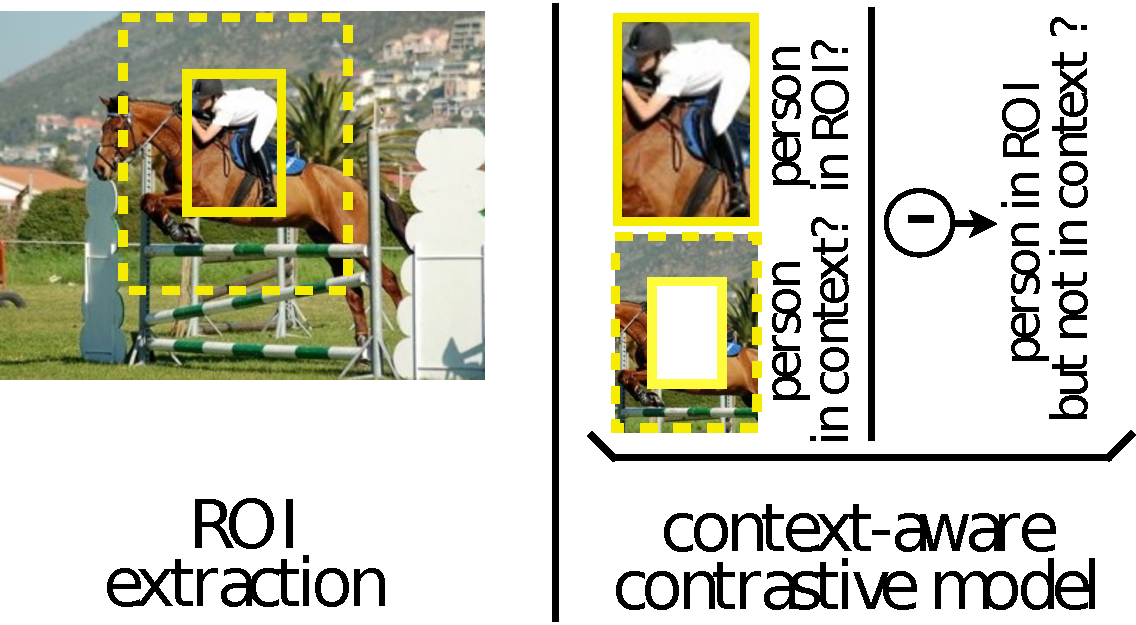
\includegraphics[width=\textwidth, trim={2mm 6.0cm 20mm 3cm},clip]{images/overview}
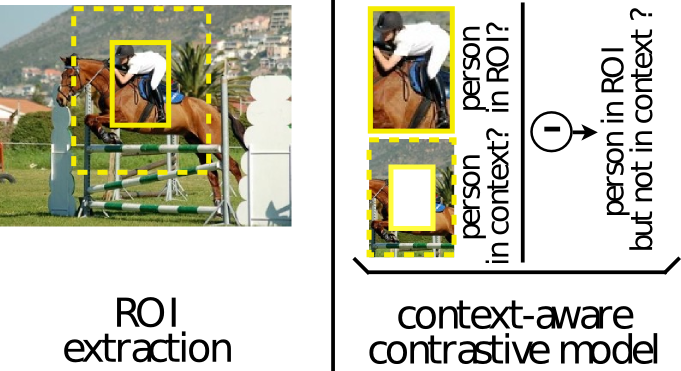
\includegraphics[width=\textwidth,clip]{images/overview.png}
\end{center}
			\end{block}
		\end{mdframed}

	 \begin{block}{Contributions}
		\begin{itemize}
			\item Explore context-aware ConvNet models for weakly supervised localization (WSL)
			\item Propose a novel context-aware contrastive model for WSL
			\item Demonstrate its effectiveness on PASCAL VOC 2007 / 2012
			\item State of the art on the datasets for models with same base architecture
		\end{itemize}
		
	 \end{block}

\begin{block}{Task definitions}
		\begin{itemize}
			\item Object localization: for a given class label find the most confident tight bounding box
			\item Object detection: for a given class label find tight bounding boxes for all object instances
			\item Weakly supervised localization (WSL): localization with only image-level labels at train time
			\item Evaluated by detection mAP and CorLoc
		\end{itemize}
\end{block}
	 
	 \begin{block}{Related work}
		\scriptsize
		\bibliographystyle{amsalpha}
		\bibliography{shortstrings,contextlocnet_eccv2016_poster}
	\end{block}
	\end{column}
	\postercolumnbreak

\begin{column}{.44\linewidth}
	\definecolor{color_conv_fc}{HTML}{96D35F}
	\definecolor{color_region_pooling}{HTML}{FFB5AF}
	\definecolor{color_classification_stream}{HTML}{FAEA99}
	\definecolor{color_localization_stream}{HTML}{CAE4FD}
	
	\begin{block}{Approach}
		\def \columnsizemodel {.35\linewidth}
		\def \columnsizedescr {.65\linewidth}
		\def \increaseitemsep {\setlength\itemsep{1cm}}
		\def \modelsep {\bigskip\bigskip\bigskip}
		
		\begin{center}
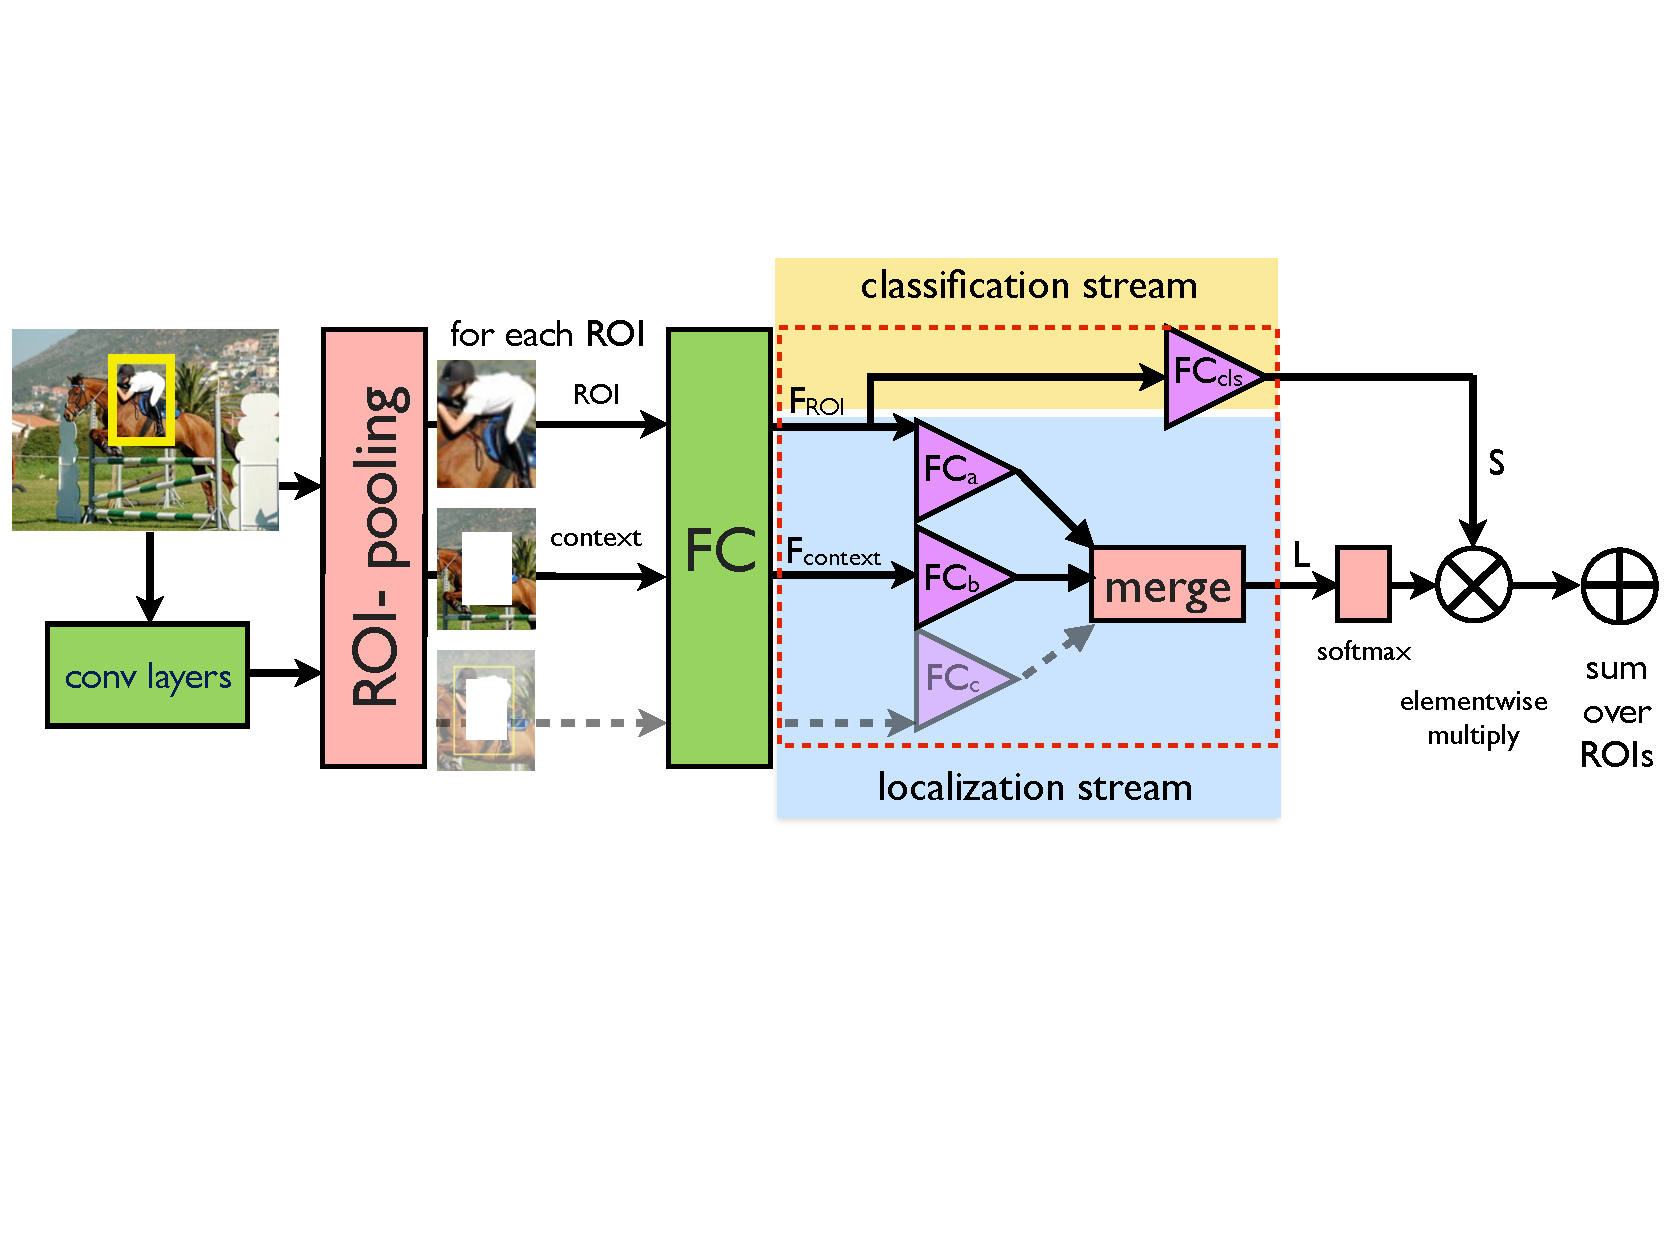
\includegraphics[width=\textwidth, trim={1mm 7.3cm 1mm 4cm},
clip]{images/model}
\end{center}
		\begin{itemize}
			\increaseitemsep
			%\item In train time, image-level labels are encoded as $y \in \{1, -1\}^C$ where $C$ is the number of classes
			\item Each image is passed through \colorbox{color_conv_fc}{conv layers} (VGG-F).
			\item $K$ selective search proposals (SSW) are generated for each image.
			\item For each proposal, \colorbox{color_region_pooling}{region pooling}~\cite{Gidaris:2015cx} performs feature pooling with different shapes: ROI, context, frame. 	
			\end{itemize}
		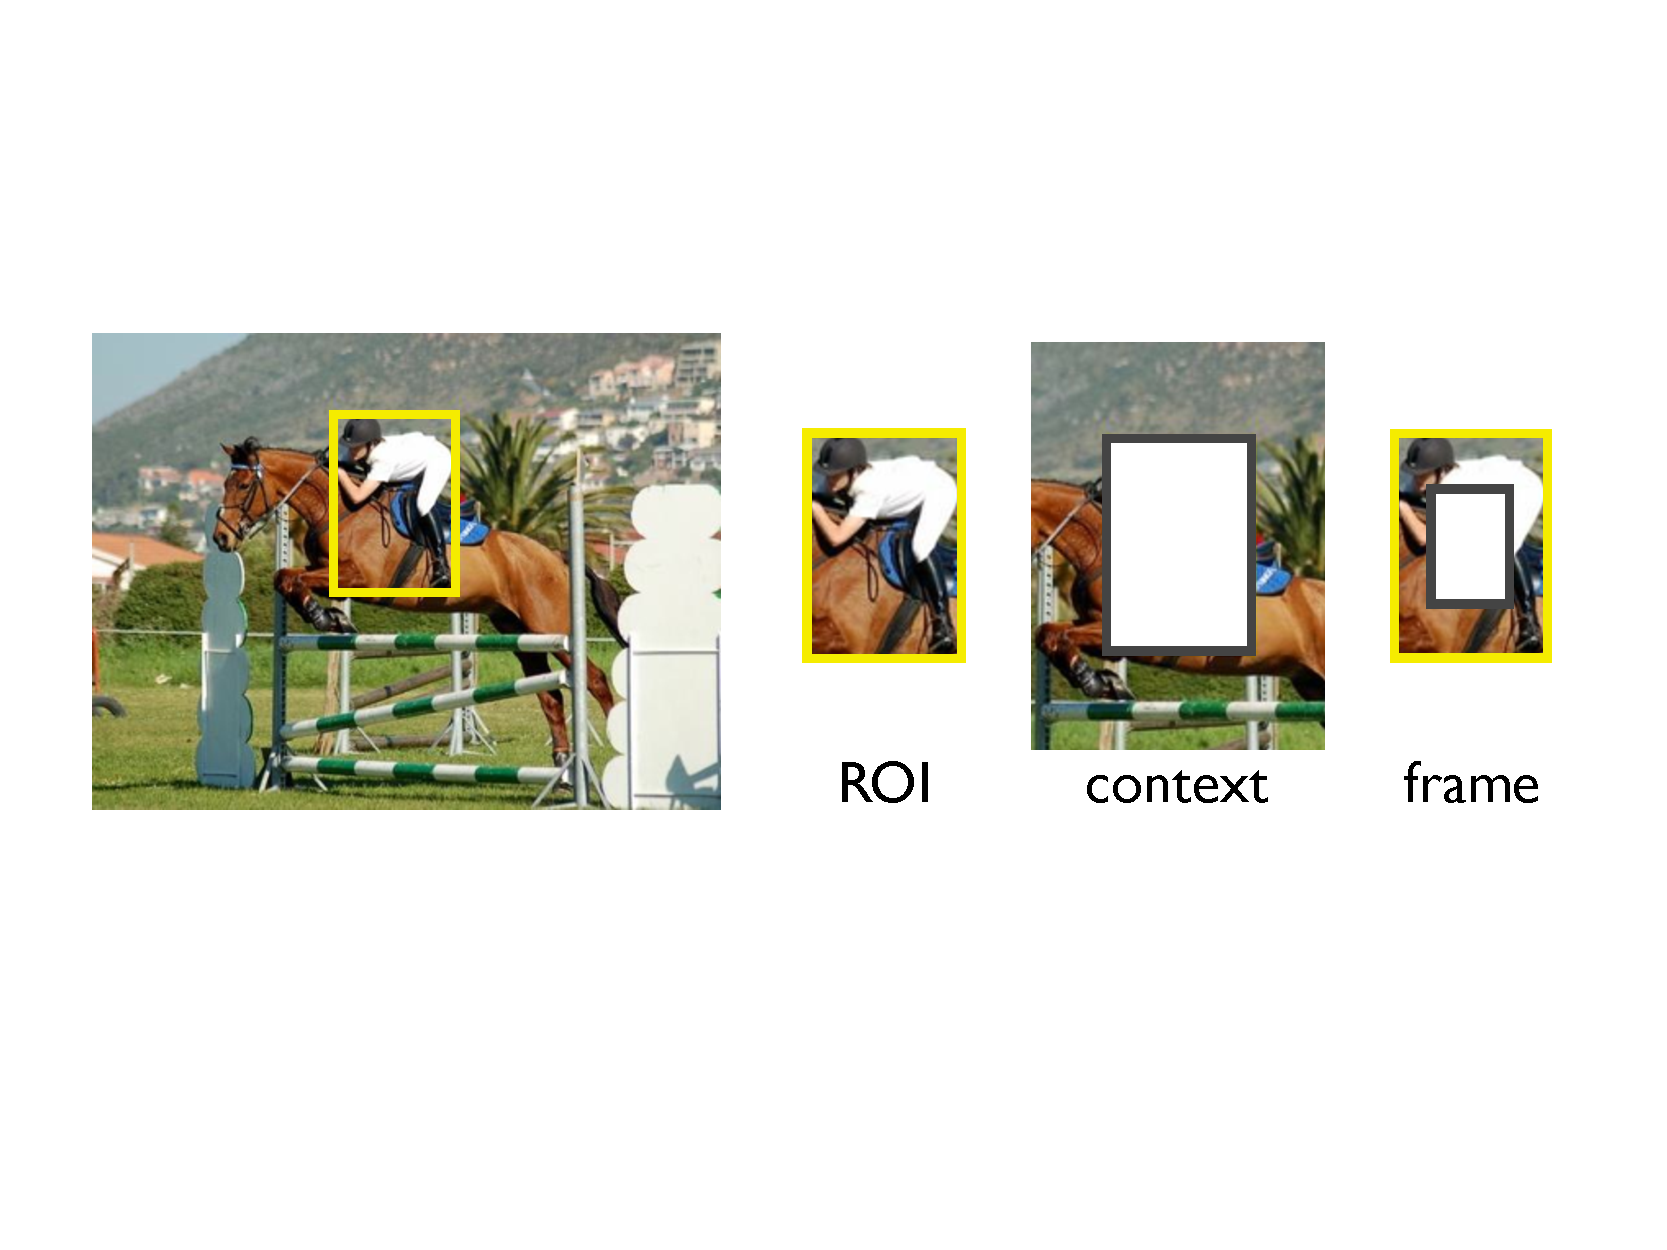
\includegraphics[width=\textwidth, trim={1mm 7.5cm 1mm 5cm},
clip]{images/roitransforms}
		\bigskip\bigskip
		\begin{itemize}
			\increaseitemsep
			\item \colorbox{color_conv_fc}{FC} (fully-connected) layer takes the pooling results,  produces features $F_{\rm ROI}$, $F_{\rm context}$, $F_{\rm frame}$, and feeds them into two streams, inspired by~\cite{Bilen:2015uo}.
			\item \colorbox{color_classification_stream}{Classification stream} produces a matrix of classification scores $S = [{\rm FC_{cls}}(F_{\rm ROI_1}); \dots; {\rm FC_{cls}}(F_{\rm ROI_K})] \in \mathbb{R}^{K \times C}$
			\item \colorbox{color_localization_stream}{Localization stream} implements the proposed context-aware guidance that uses $F_{\rm ROI_k}$, $F_{\rm context_k}$, $F_{\rm frame_k}$ to produce a localization score matrix $L \in \mathbb{R}^{K \times C}$.
		\end{itemize}
		
		\modelsep
		\begin{columns}[T,onlytextwidth]
			\begin{column}{\columnsizemodel}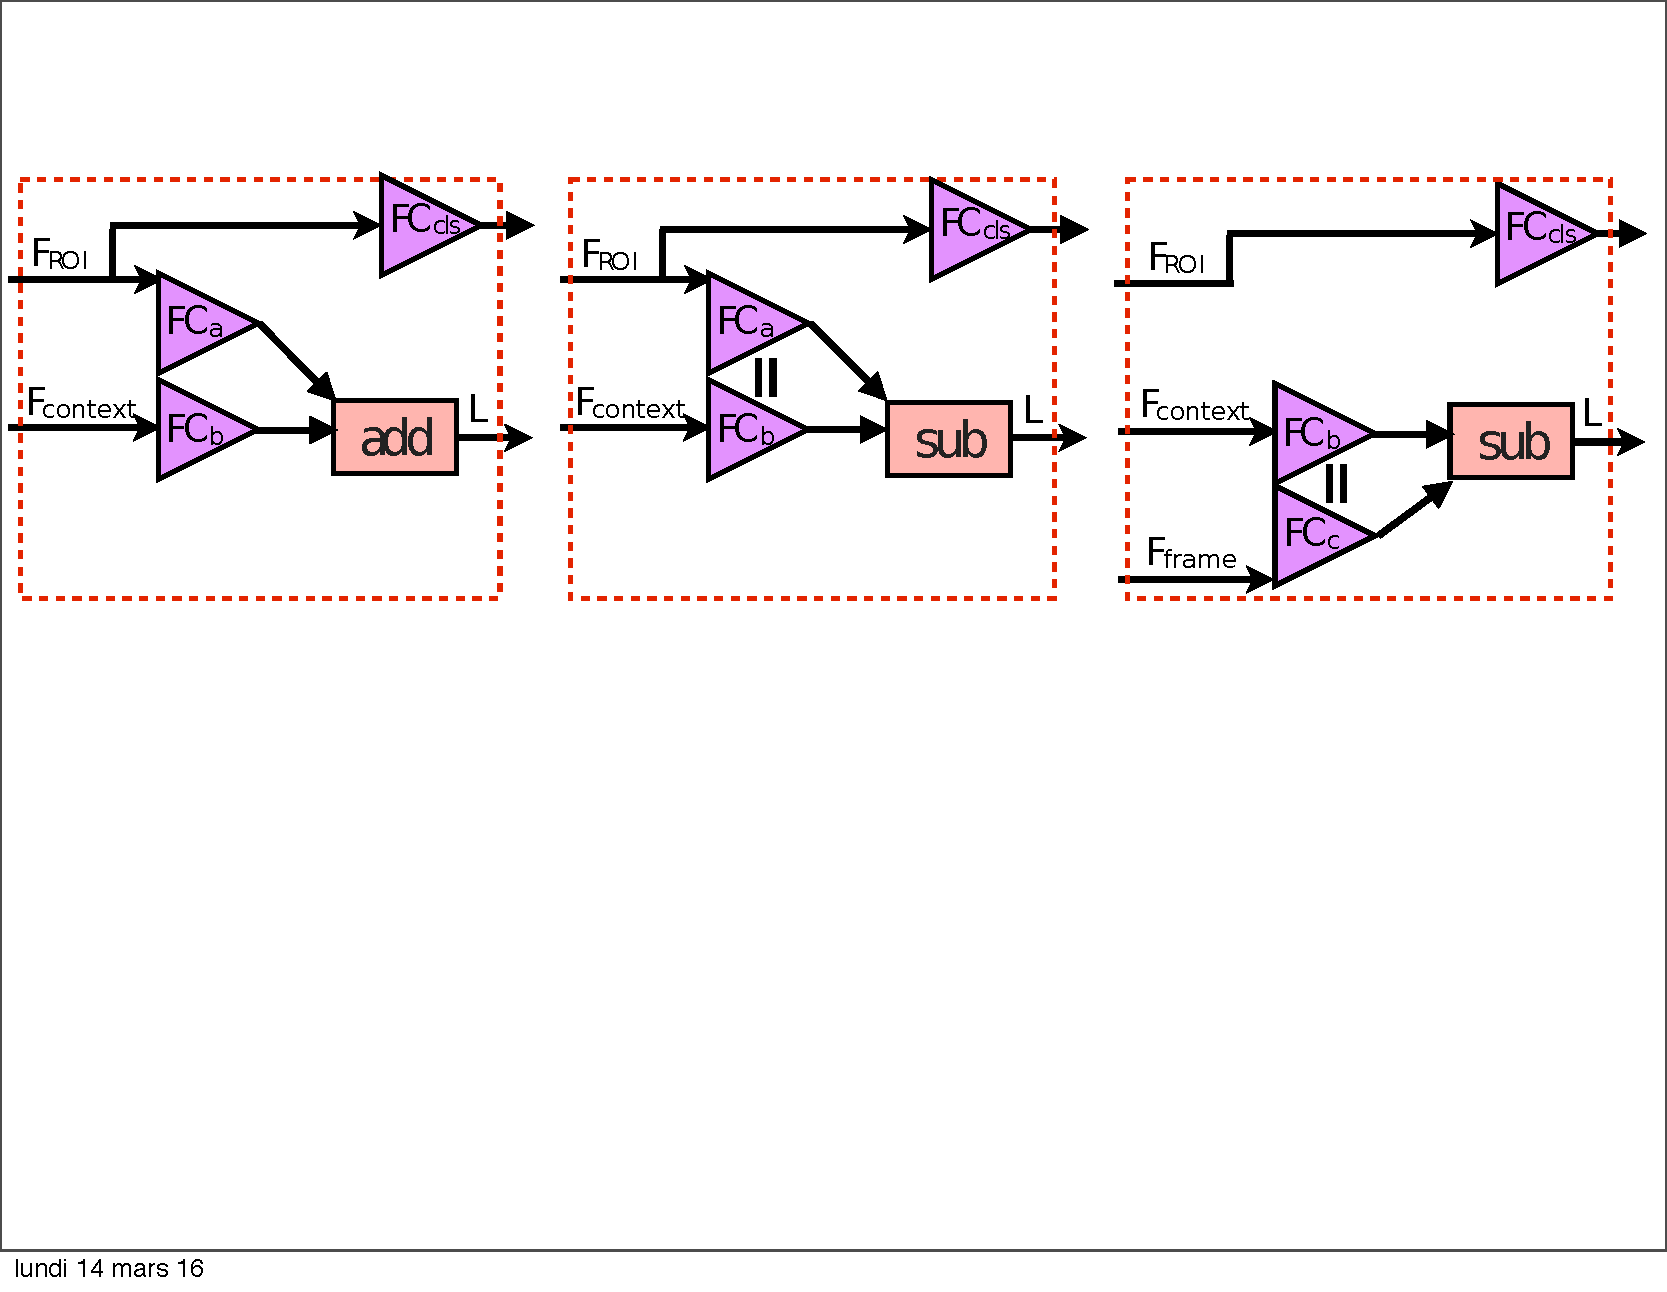
\includegraphics[width=\textwidth, trim={19cm 11cm 1mm 2.8cm},clip]{images/variants-horiz}\end{column}
			\begin{column}{\columnsizedescr}
				\begin{block}{\small Contrastive model S}
				\vspace{-0.5cm}
				\begin{itemize}
					\item Trains a single fully-connected layer ${\rm FC_{contrast}}$.
					\item Computes contrast between class activations of proposal and its context.
					\item Uses $F_{\rm frame_k}$ instead of $F_{\rm ROI_k}$ to ensure consistency of inputs to ${\rm FC_{contrast}}$.
					\item $L_{kc} = {\rm FC_{contrast}^{c}}(F_{\rm frame_k}) - {\rm FC_{contrast}^{c}}(F_{\rm context_k})$
				\end{itemize}
				\end{block}
			\end{column}
		\end{columns}
		
		\modelsep
		\begin{columns}[T,onlytextwidth]
			\begin{column}{\columnsizemodel}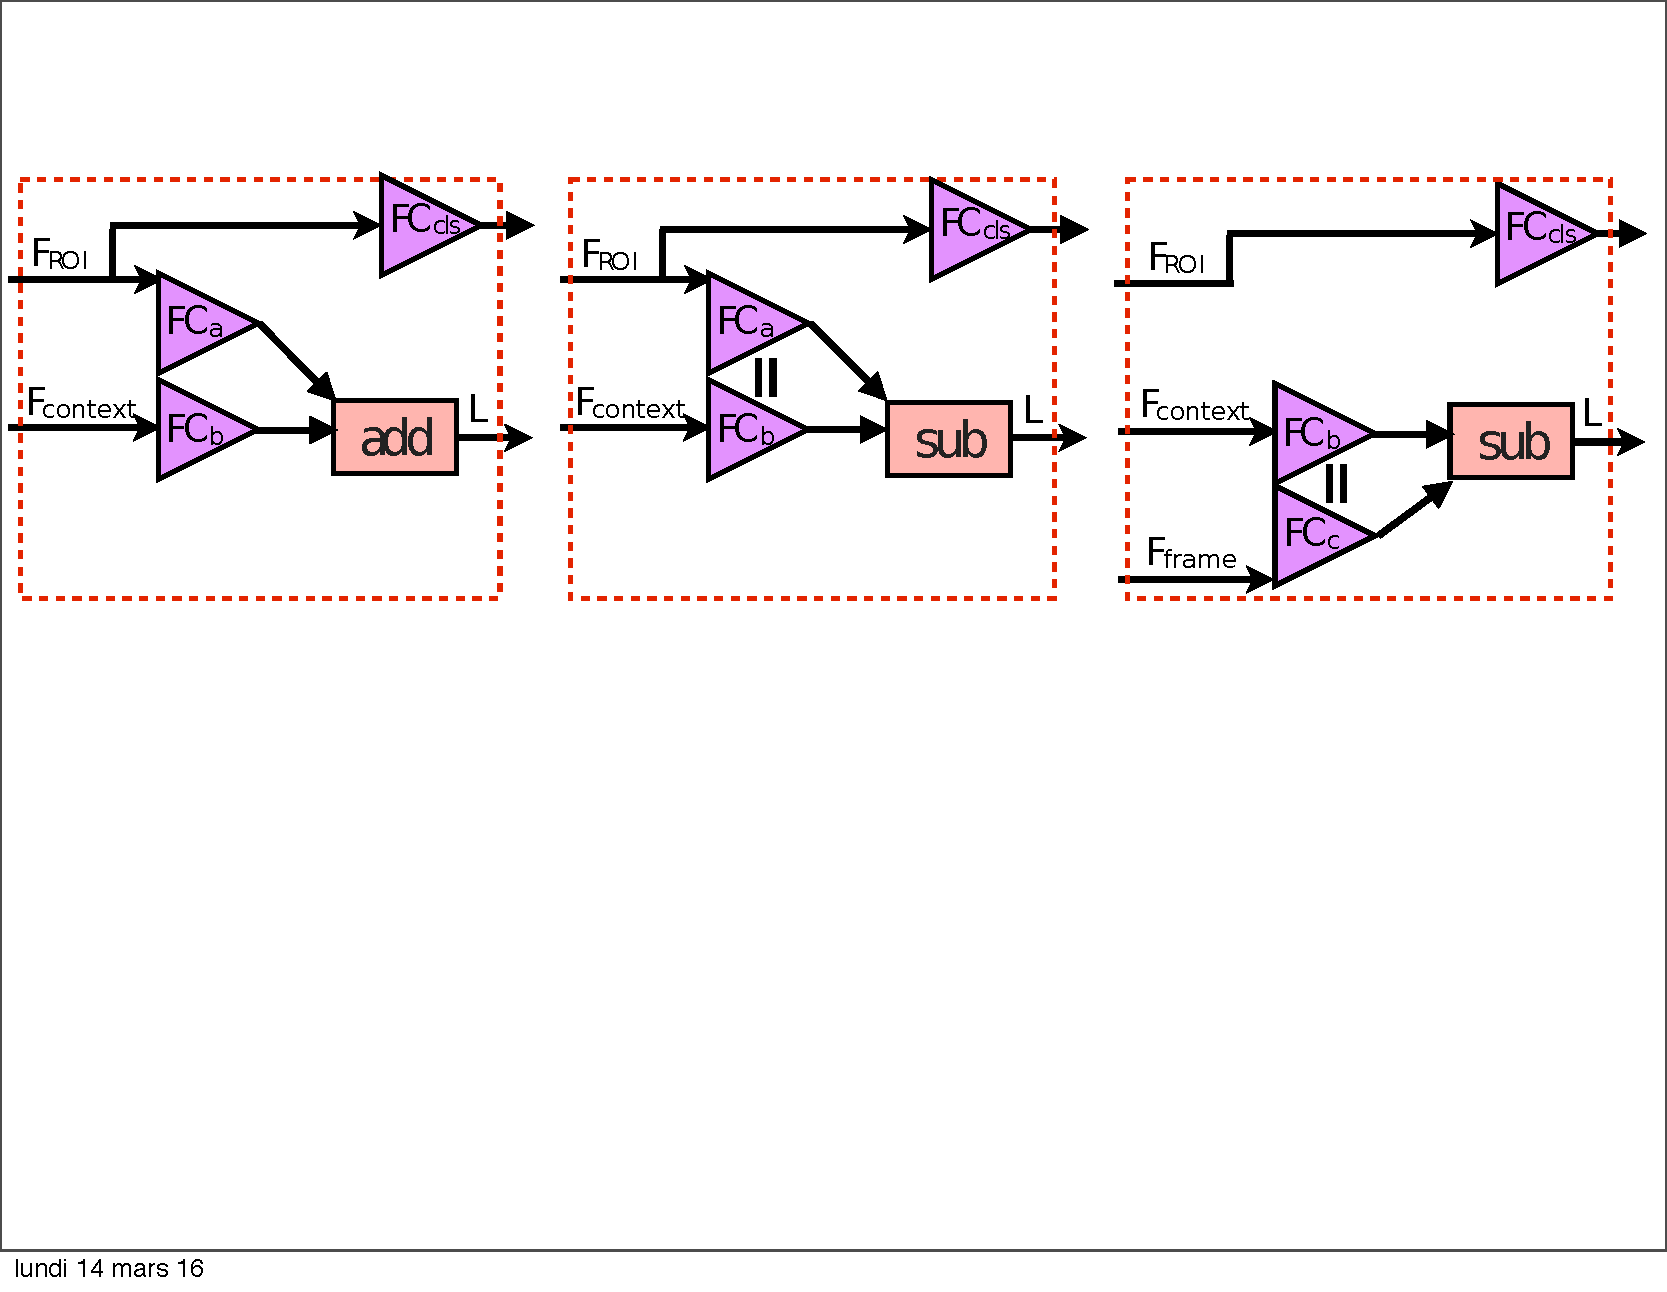
\includegraphics[width=\textwidth, trim={9.5cm 11cm 9.5cm 2.8cm},clip]{images/variants-horiz}\end{column}
			\begin{column}{\columnsizedescr}
				\begin{block}{\small Contrastive model A}
				\begin{itemize}
					\item Trains a simpler contrastive model using ROI and context.
					\item $L_{kc} = {\rm FC_{contrast}^{c}}(F_{\rm ROI_k}) - {\rm FC_{contrast}^{c}}(F_{\rm context_k})$
				\end{itemize}
				\end{block}
			\end{column}
		\end{columns}
		
		\modelsep
		\begin{columns}[T,onlytextwidth]
			\begin{column}{\columnsizemodel}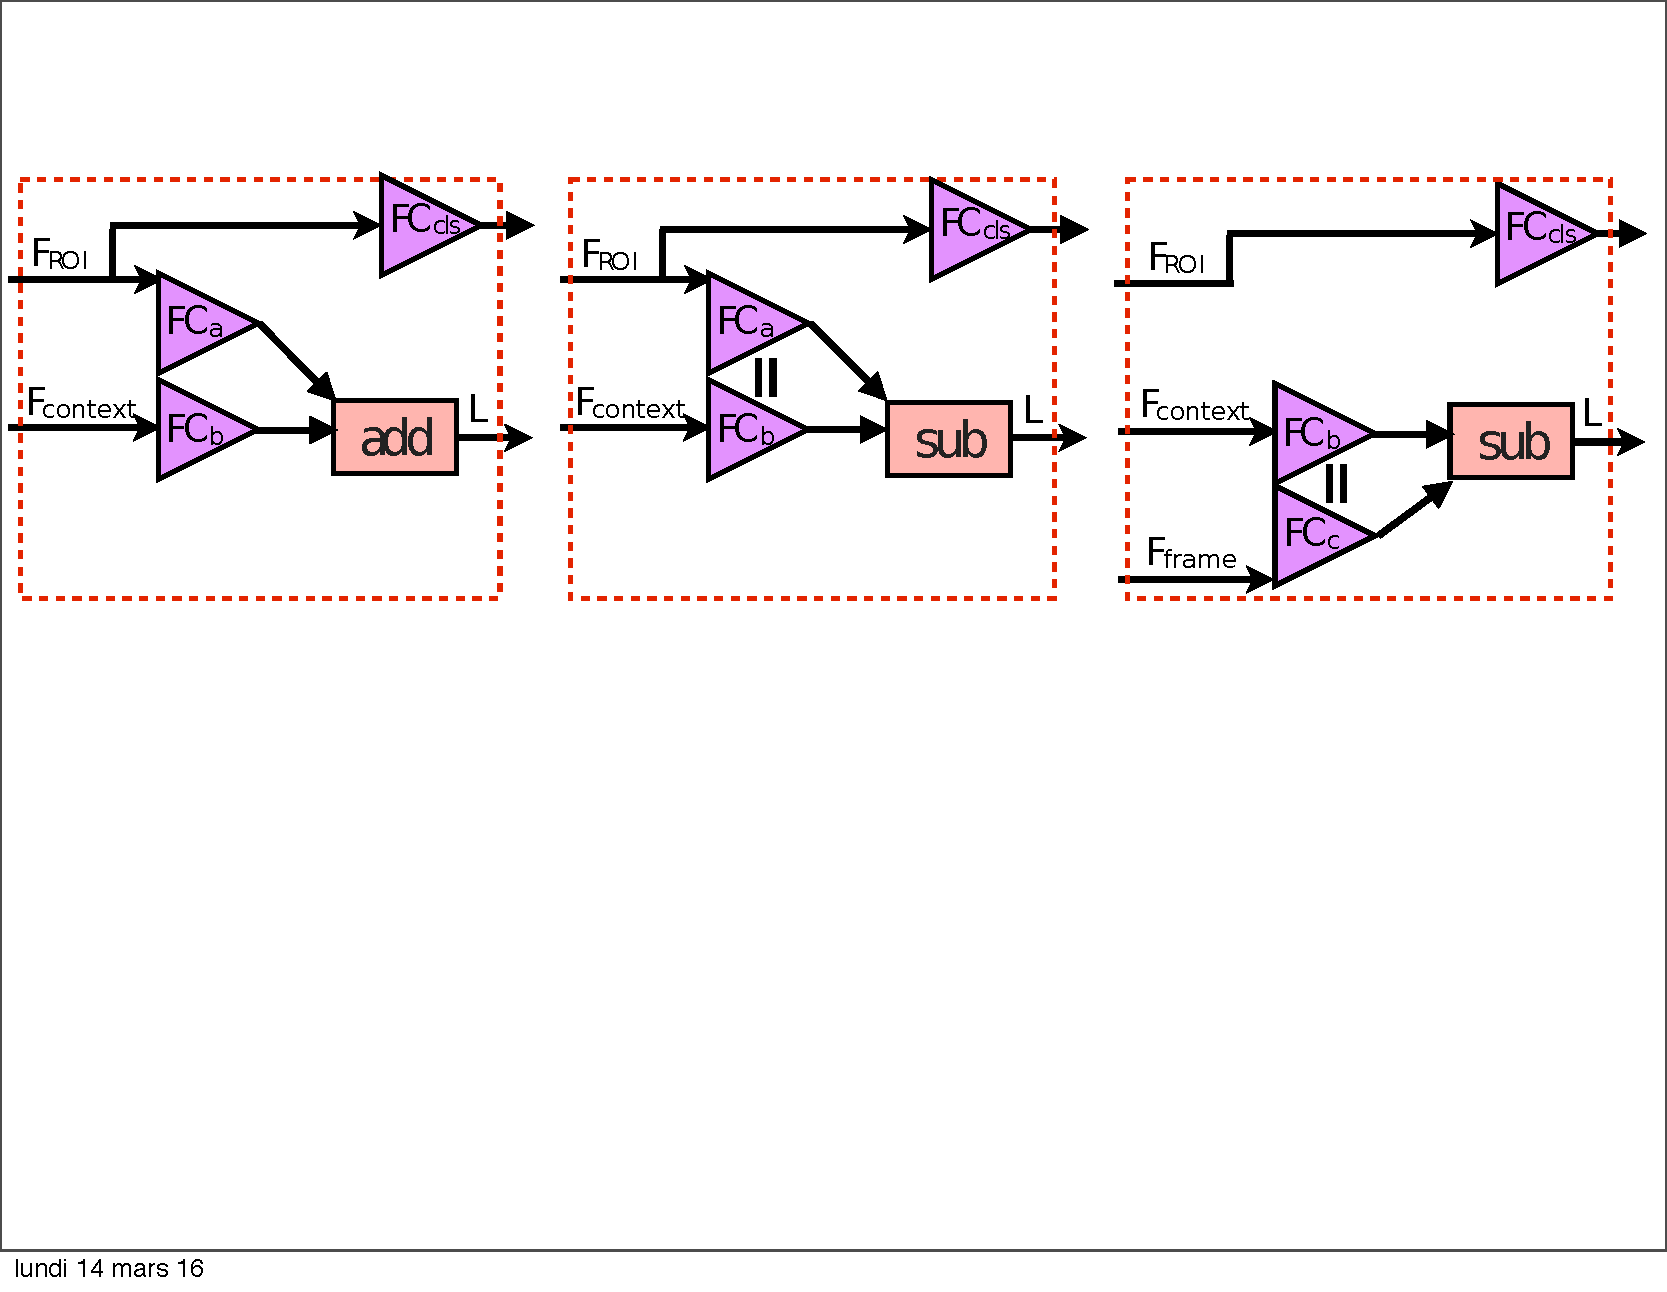
\includegraphics[width=\textwidth, trim={1mm 11cm 19cm 2.8cm},clip]{images/variants-horiz}\end{column}
			\begin{column}{\columnsizedescr}
				\begin{block}{\small Additive model}
				\begin{itemize}
					\item Trains two fully-connected layers ${\rm FC_{ROI}}$ and ${\rm FC_{context}}$ to select a proposal that is semantically compatible with its context.
					\item $L_{kc} = {\rm FC_{ROI}^{c}}(F_{\rm ROI_k}) + {\rm FC_{context}^{c}}(F_{\rm context_k})$
				\end{itemize}
				\end{block}
			\end{column}
		\end{columns}
		\modelsep
		
		\begin{itemize}
			\increaseitemsep
			\item The subsequent softmax layer normalizes the scores over all ROIs in the image:  $ [ \sigma(L) ]_{kc} = \frac{\exp(L_{kc})}{\sum_{k'=1}^{K}{\exp(L_{k'c})}}$. 
			\item Final score for each proposal and class is obtained by element-wise multiplication of the corresponding scores $S$ and $\sigma(L)$.
			\item Final image score $f_c(x)$ for each class $c$ is a sum of these proposal scores.
			\item \colorbox{color_conv_fc}{Conv} and \colorbox{color_conv_fc}{FC} layers are initialized with VGG-F. All layers are trained with hinge loss $J(x, y) = \frac{1}{C}\sum_{c=1}^{C}\max(0, 1 - y_{ci} \cdot f_c(x_i; w))$.
		\end{itemize}
	
	\end{block}
	
	\begin{mdframed}[style = posteremphasize]
	\begin{block}{Torch code is online}
		\centering \url{http://www.di.ens.fr/willow/research/contextlocnet}
	\end{block}
	\end{mdframed}
\end{column}

\postercolumnbreak

\begin{column}{.26\linewidth}
	\begin{block}{Results on VOC 2007}
		{\small %%
\begin{center}
\begin{tabular}{llcc}
\toprule
Model &  CorLoc & mAP \\
\midrule
\cite{Cinbis:2015wn}  &52.0&30.2\\
\cite{Wang:2014tg} & 48.5 & 30.9 \\
\cite{Wang:2014tg} + context &&31.6\\
WSDDN-SSW-S \cite{Bilen:2015uo}&      & 31.1       \\
WSDNN-SSW-ENS \cite{Bilen:2015uo} & 54.2 & 33.3\\
\midrule
WSDDN-SSW-S$^*$& 50.0      & 30.5       \\
additive & 52.8      & 33.3       \\
contrastive A & 50.2      & 32.2       \\
contrastive S & \textbf{55.1}      & \textbf{36.3}       \\



%%
%%
%%
%%
%%
%%
%%
%%
\bottomrule
\end{tabular}
\end{center}
}
		\begin{itemize}
			\item VOC 2007: 5k trainval images, 5k test images, 20 classes
			\item WSDDN-SSW-S$^*$ is our reimplementation of~\cite{Bilen:2015uo}.
			\item Contrastive model S outperforms the baseline~\cite{Bilen:2015uo}.
			\item About 1\% variance for all models measured over 5 runs.
		\end{itemize}
	\end{block}
	
	\begin{block}{Results on VOC 2012}
		{\footnotesize \begin{center}
\begin{adjustbox}{max width=1.02\textwidth}
\begin{tabular}{l@{\hskip 0.5cm}c*{20}cc}
\toprule
&  aer & bik & brd & boa & btl \\
contrastive S (CorLoc) & 78.3 & 70.8 & 52.5 & 34.7 & 36.6 \\
contrastive S (mAP) & 64.0 & 54.9 & 36.4 & 8.1 & 12.6 \\
\midrule

& bus & car & cat & cha & cow \\
contrastive S (CorLoc) & 80.0 & 58.7 & 38.6 & 27.7 & 71.2 \\
contrastive S (mAP) &  53.1 & 40.5 & 28.4 & 6.6 & 35.3 \\

\midrule
& tbl & dog & hrs & mbk & prs \\
contrastive S (CorLoc) & 32.3 & 48.7 & 76.2 & 77.4 & 16.0 \\
contrastive S (mAP) & 34.4 & 49.1 & 42.6 & 62.4 & 19.8 \\

\midrule
& plt & shp & sfa & trn & tv & Avg. \\
contrastive S (CorLoc) & 48.4 & 69.9 & 47.5 & 66.9 & 62.9 & \textbf{54.8} \\
contrastive S (mAP) & 15.2 & 27.0 & 33.1 & 33.0 & 50.0 & \textbf{35.3}  \\
\bottomrule

%\toprule
%Model &  aer & bik & brd & boa & btl & bus & car & cat & cha & cow &
%tbl & dog & hrs & mbk & prs & plt & shp & sfa & trn & tv & Avg. \\
%\midrule
%contrastive S (mAP) & 64.0 & 54.9 & 36.4 & 8.1 & 12.6 & 53.1 & 40.5 & 28.4 & 6.6 & 35.3 & 34.4 & 49.1 & 42.6 & 62.4 & 19.8 & 15.2 & 27.0 & 33.1 & 33.0 & 50.0 & 35.3 \\
%contrastive S (CorLoc) & 78.3 & 70.8 & 52.5 & 34.7 & 36.6 & 80.0 & 58.7 & 38.6 & 27.7 & 71.2 & 32.3 & 48.7 & 76.2 & 77.4 & 16.0 & 48.4 & 69.9 & 47.5 & 66.9 & 62.9 & 54.8 \\
%\bottomrule

\end{tabular}

\end{adjustbox}

\end{center}
}
		\begin{itemize}
			\item VOC 2012: 11k trainval images, 11k test images, 20 classes
		\end{itemize}
	\end{block}
	
	\begin{block}{Example detections}
		\begin{center}
			\footnotesize{Contrastive S improves over WSDDN-SSW-S$^*$}
			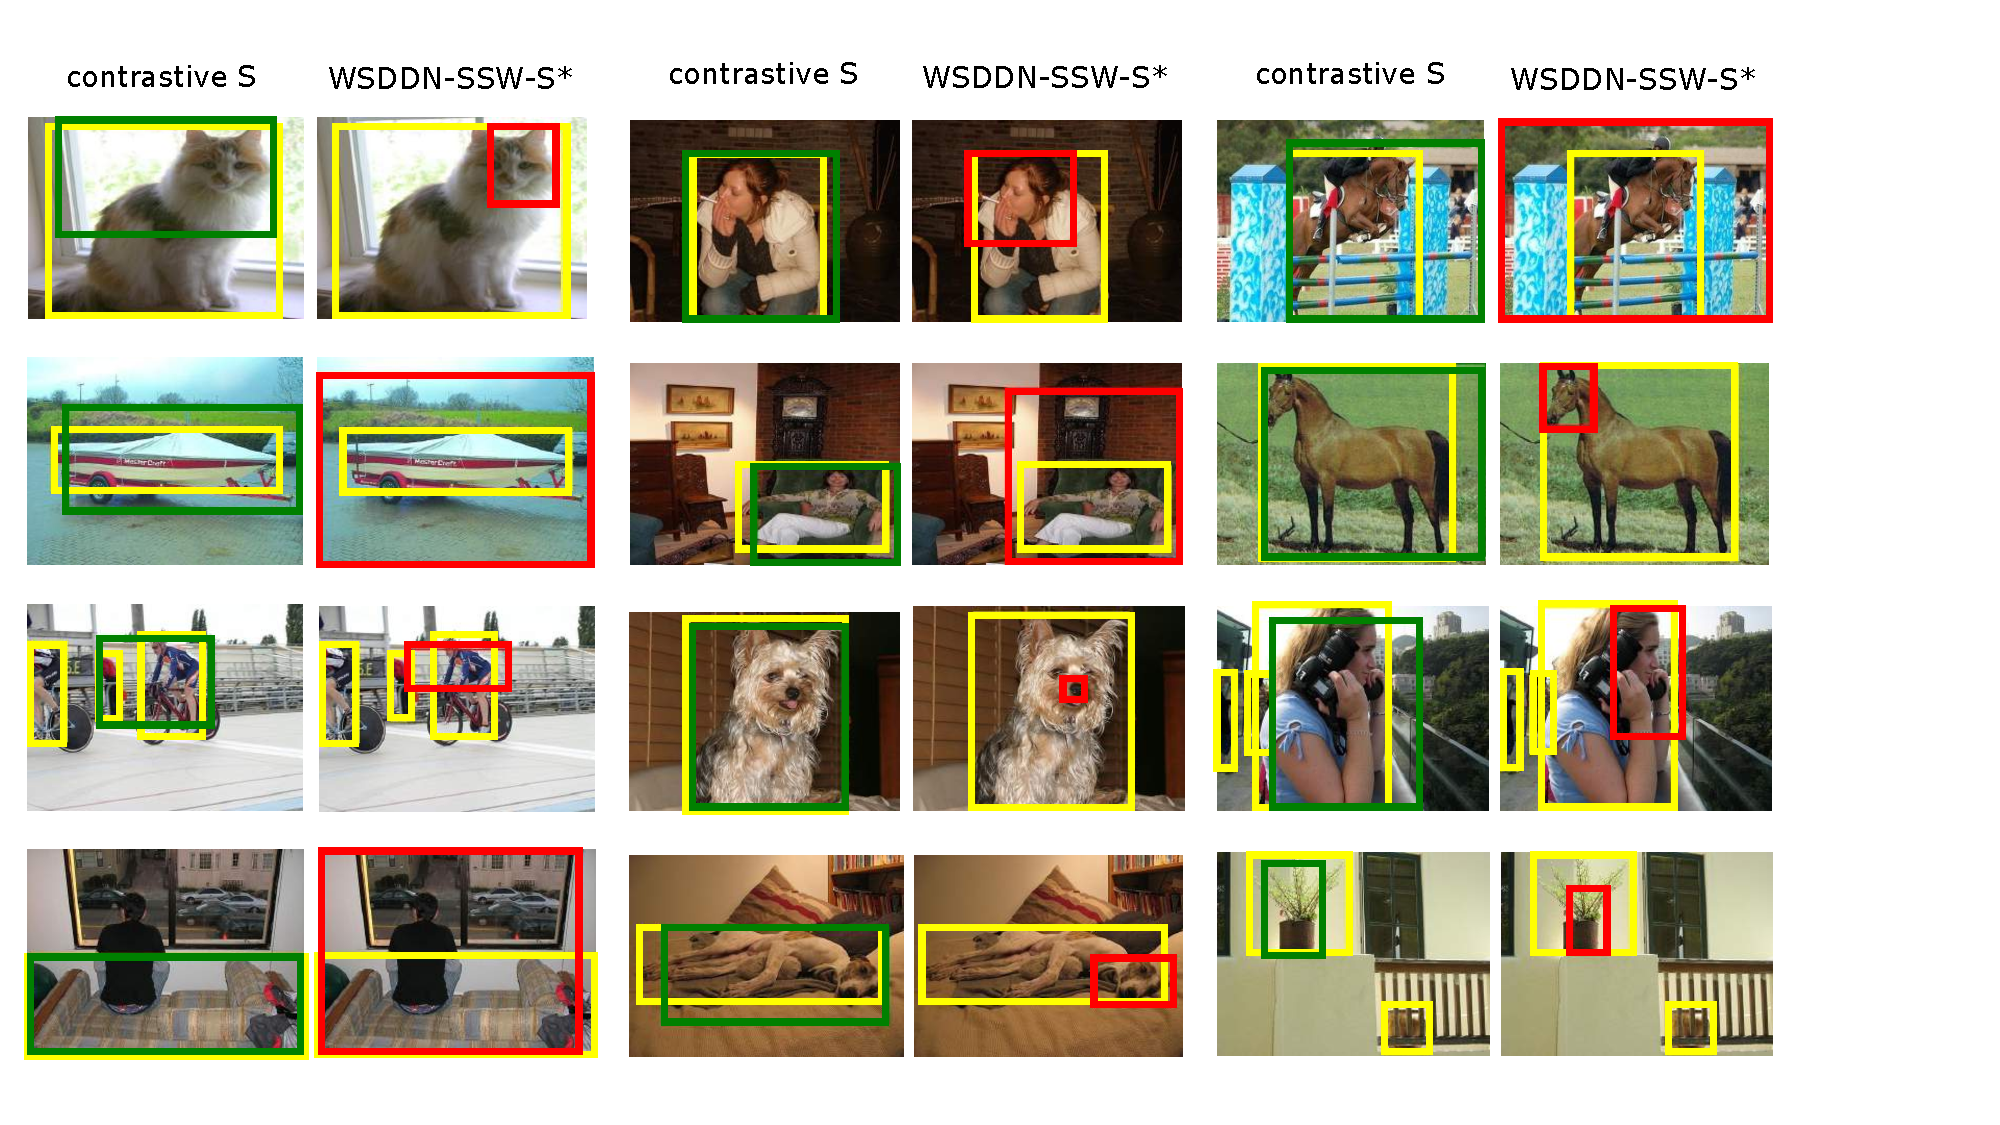
\includegraphics[trim = 0cm 0.8cm 2.8cm 0cm, clip, width=0.98\linewidth] {images/detectionresults_goodbad_1_compressed.pdf}

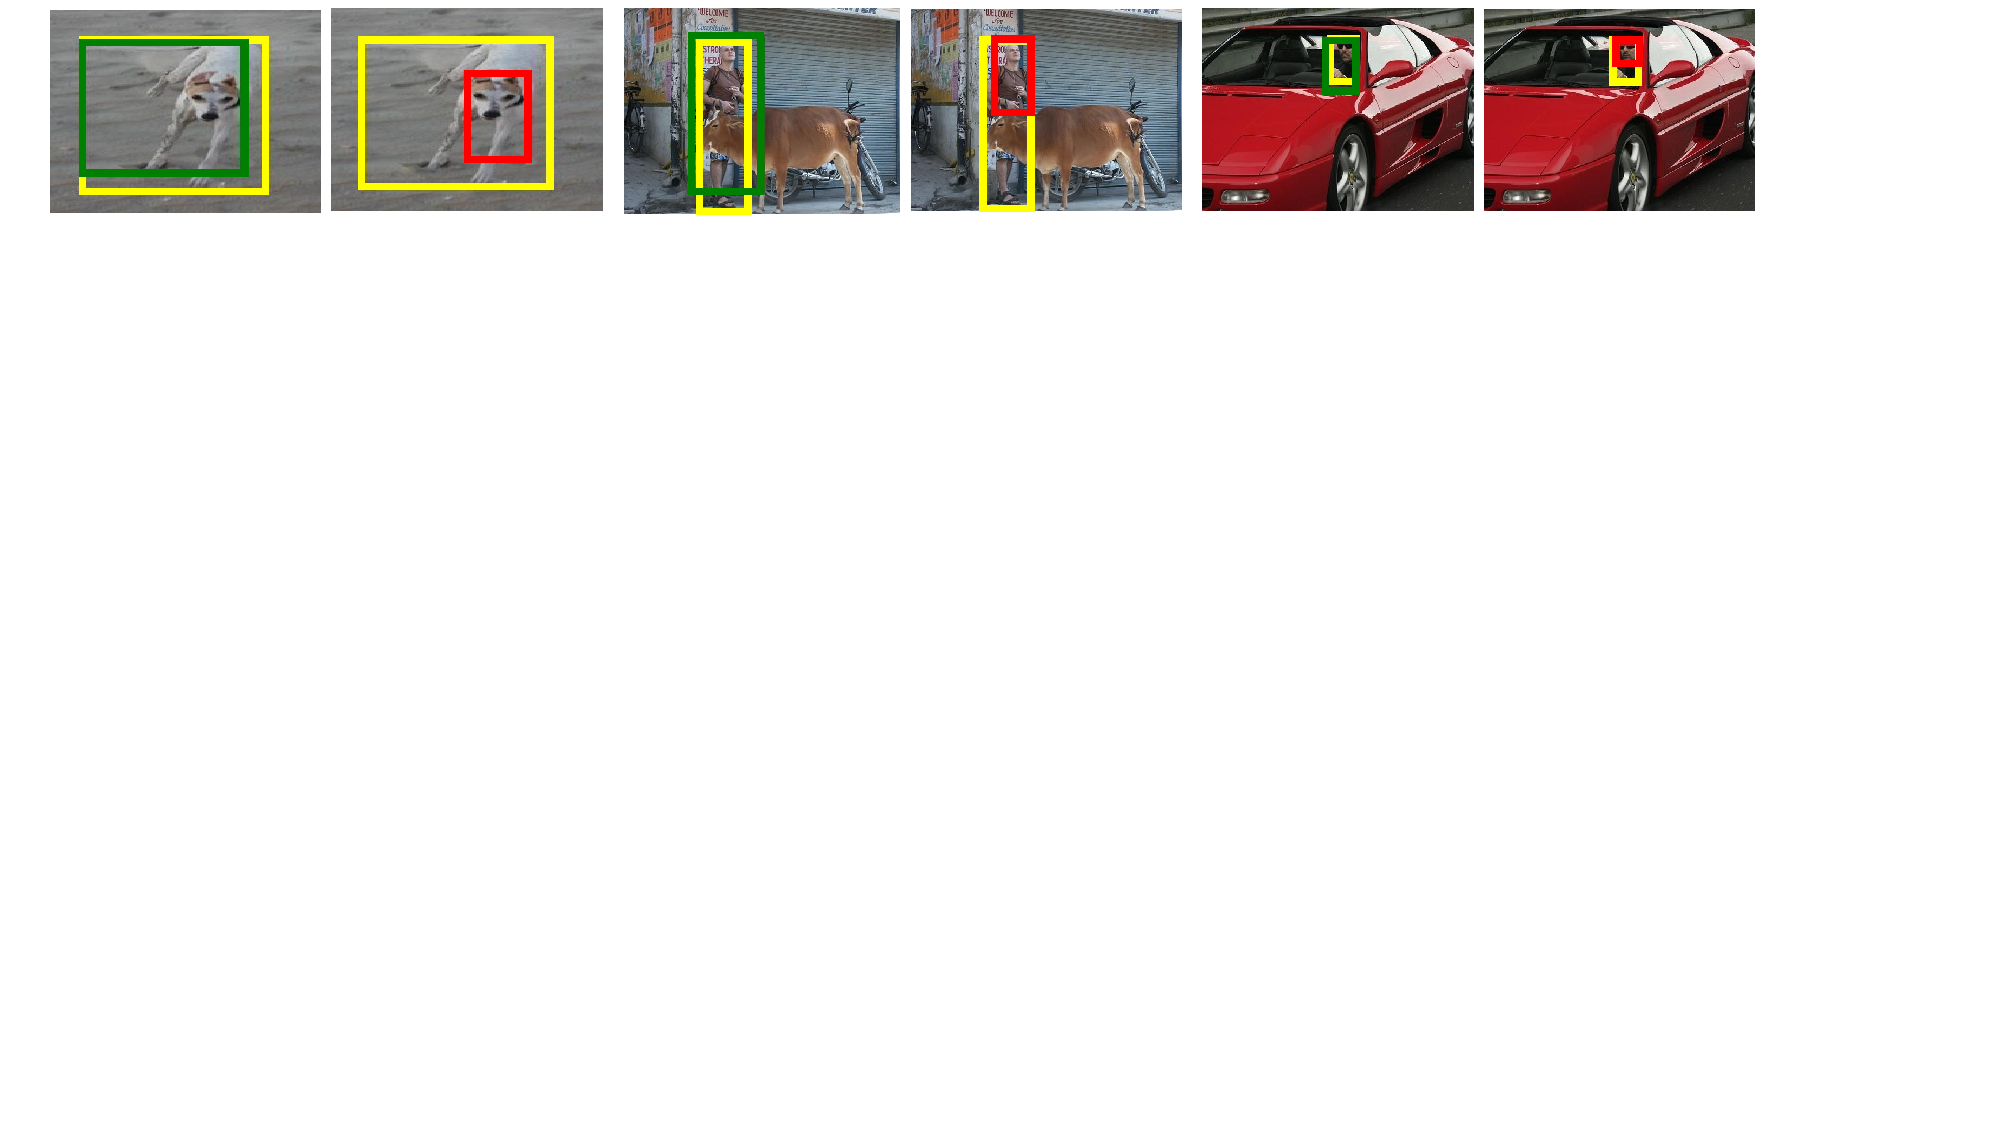
\includegraphics[trim = 0cm 15.5cm 2.8cm 0cm, clip, width=1.0\linewidth] {images/detectionresults_goodbad_4.pdf}

		
			\footnotesize{Success of both models}
			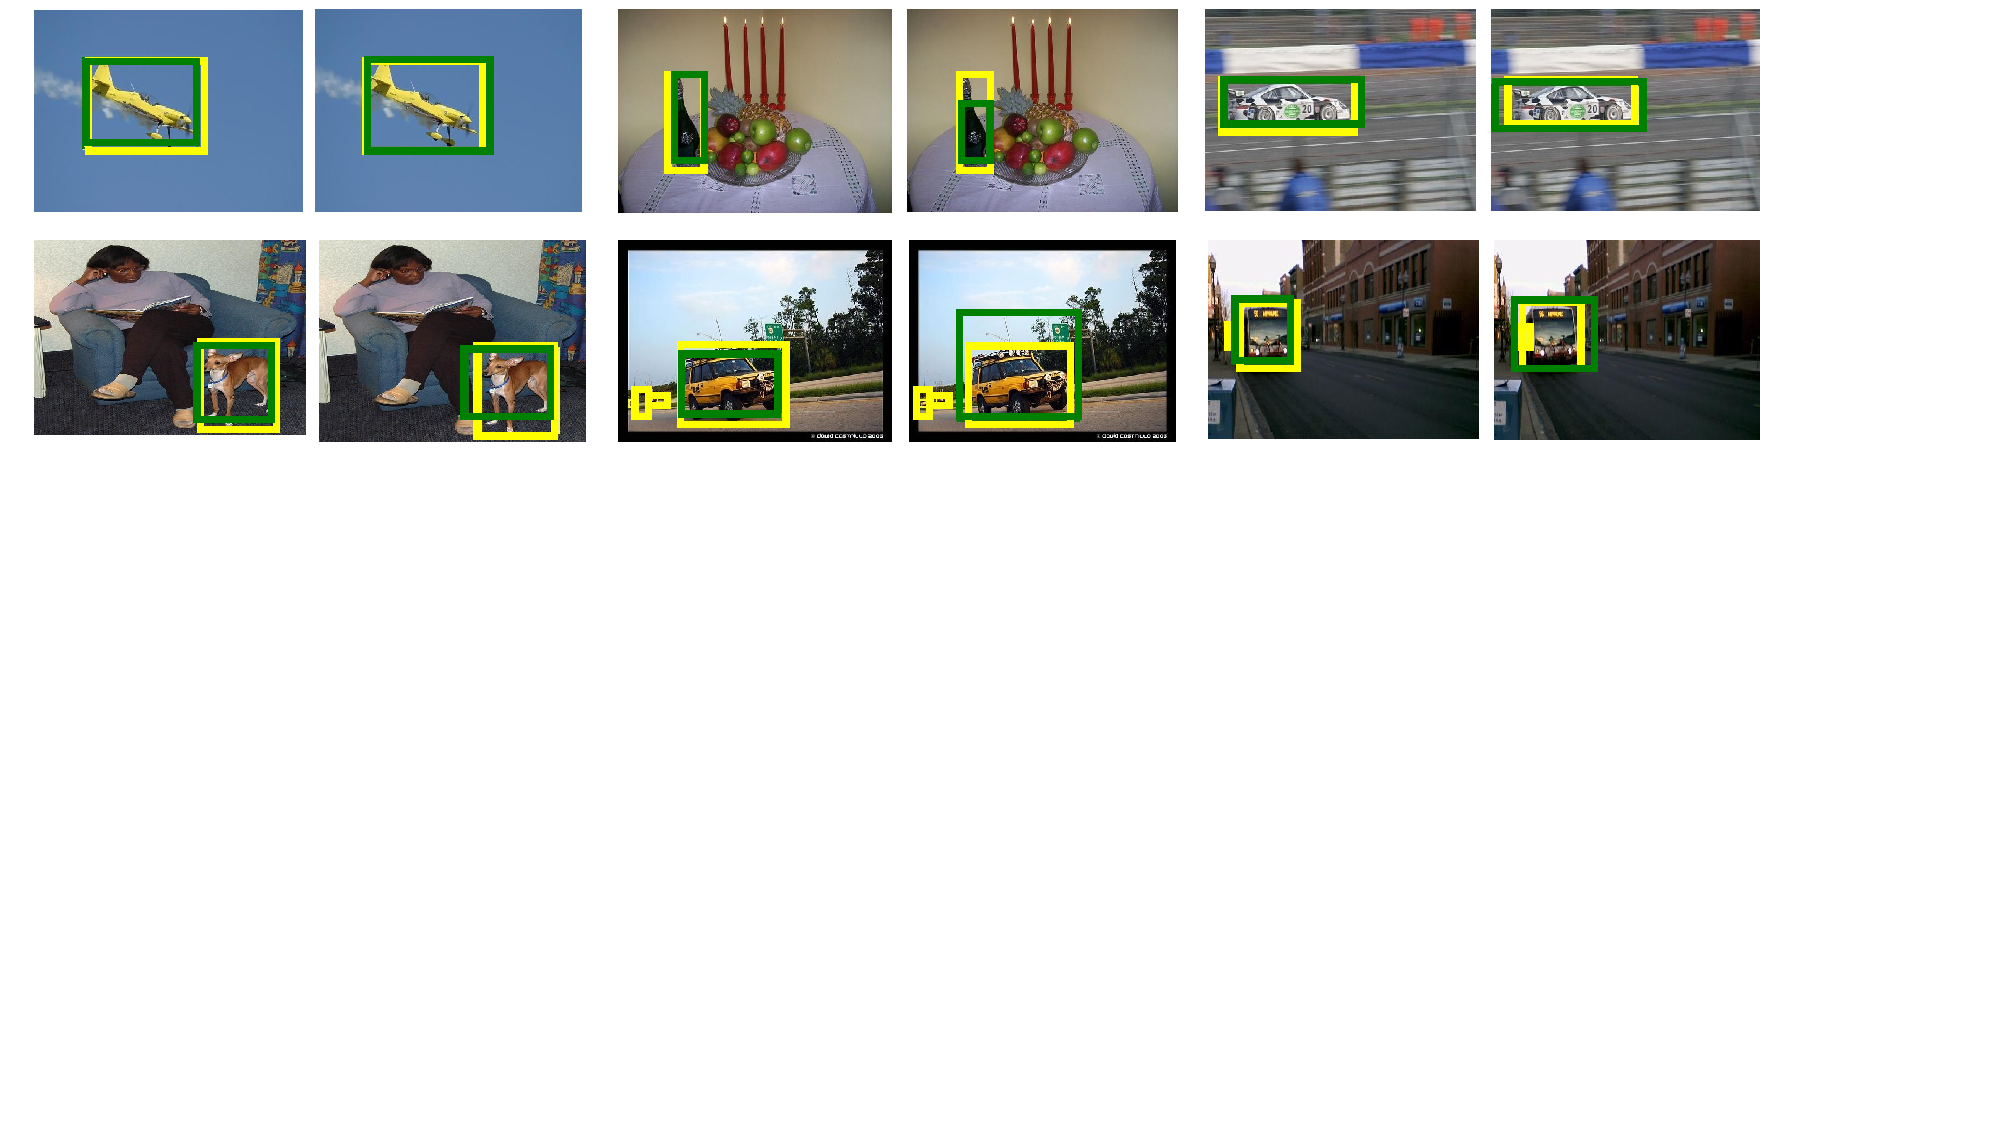
\includegraphics[trim = 0cm 11cm 3cm 0cm, clip, width=0.985\linewidth] {images/detectionresults_goodbad_3.pdf}
		
			\footnotesize{Failure of both models}
			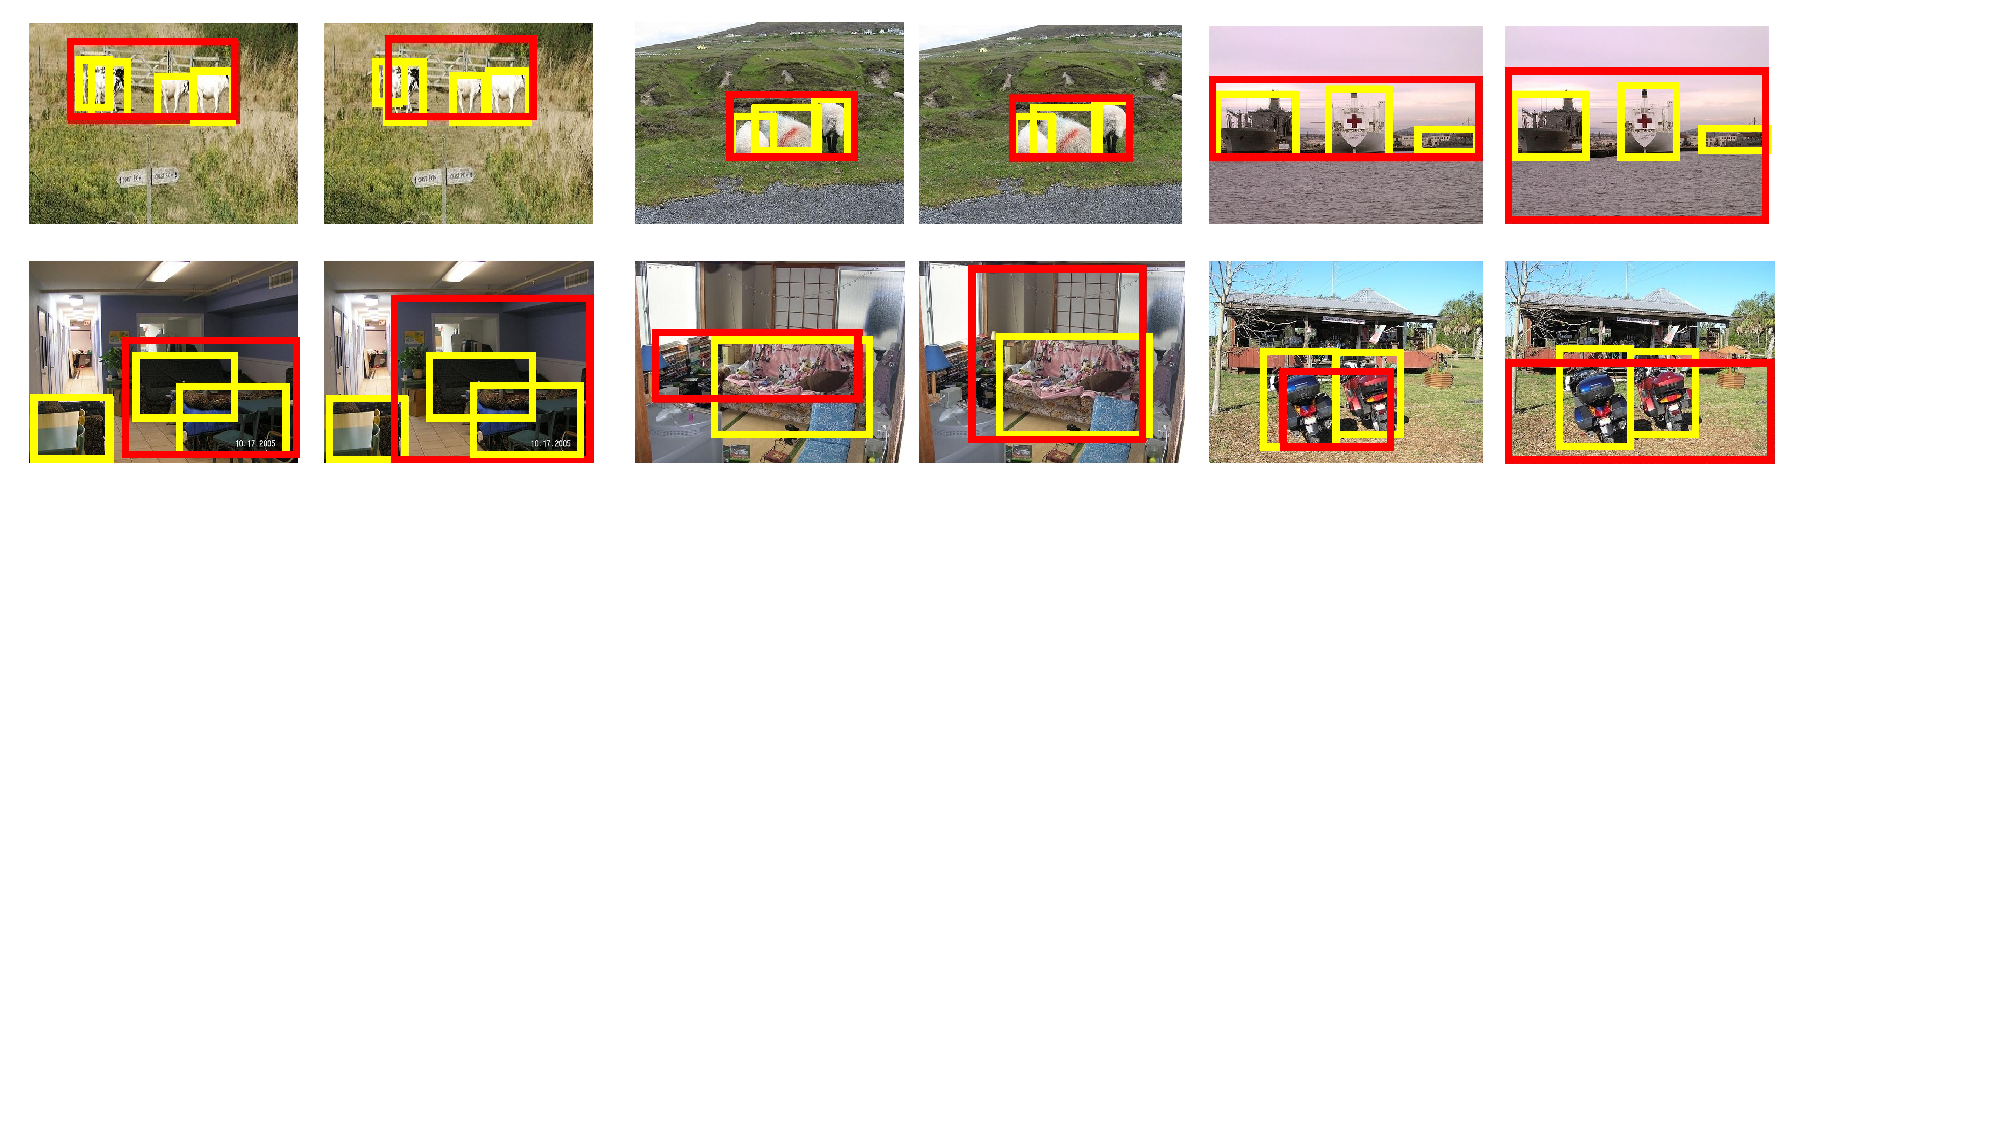
\includegraphics[trim = 0cm 11cm 3cm 0cm, clip, width=0.98\linewidth] {images/detectionresults_goodbad_2.pdf}
		\end{center}
	\end{block}
	
	\begin{block}{Conclusions}
		\begin{itemize}
			\item Contrastive model S finds tight bounding boxes when the baseline~\cite{Bilen:2015uo} fails.
			\item Failure cases include localization of overlapping instances of the same object class.
		\end{itemize}
	\end{block}
	
	\begin{block}{Implementation details}
		\begin{itemize}
			%\item VGG-F base architecture
			\item All object proposals with sides greater than 20px are used.
			\item NVIDIA Titan X single-GPU training
			\item Optimized by SGD with batch size 1, momentum $0.9$ and weight decay $5e^{-4}$
			\item $10$ epochs with learning rate $5e^{-3}$, then $20$ epochs with learning rate $5e^{-4}$
			\item Detections are filtered to have a minimum score of $10^{-4}$, then passed through NMS with threshold 0.4.
		\end{itemize}
	\end{block}
\end{column}
\end{columns}

\end{mdframed}
\end{frame}
\end{document}
